\section{\label{vqe}Variational Quantum Eigensolver}

In this chapter, we introduce the \textit{Variational Quantum Eigensolver (VQE)} algorithm, a particular class of variational quantum algorithms used to estimate the ground state energy of molecular systems. The research presented in this thesis is conducted within this framework. As providing an overview of the VQE algorithm, we will introduce the fundamentals of quantum computing and the \textit{Unitary Coupled Cluster (UCC) ansatz} used to represent fermionic wavefunctions on quantum devices.

The VQE algorithm consists of a quantum subroutine, a \textit{Parametrised Quantum Circuit (PQC)}, that implements some UCC ansatz, and a classical subroutine that classically optimises the UCC ansatz until it converges to the best approximation of the true ground state. PQCs are similar to classical neural networks in concept, but by definition, correspond to $2^n \times 2^n$ unitary maps, where $n$ is the number of qubits, and hence have the same number of inputs as outputs \cite{Yeung2020}.

The input state for the PQC is the reference state that the UCC operator $U(\bm\theta)$ acts on, which in the case of the single Slater determinant Hartree-Fock state, is encoded as a pure quantum state $\ket{\psi_0}$. The output of the PQC is then an entangled state, that is, some linear combination of vectors in the Fock space, that captures the correlation present in true ground state of the molecular system of interest.

Upon measuring the PQC output state, it collapses into a single vector in the Fock space, with a probability defined by that vector's weight in the UCC ansatz. The quantum subroutine computes the energy expectation value of the UCC ansatz via a quantum circuit consisting of the PQC and the Hamiltonian for the system.

\includezxdiagram{chapter-1/expectation}{0.7}
\begin{equation*}
    E(\bm\theta) = \bra{0} U^\dagger(\bm\theta) H U(\bm\theta) \ket{0} 
\end{equation*}

For the purposes of this thesis, we are interested in a variant of the VQE algorithm developed by Burton \textit{et al} \cite{Burton2023} known as the \textit{Discretely and Continuously Optimised Variational Quantum Eigensolver (DISCO-VQE)}. We implement a fermionic state on a quantum device as a sequence of quantum gates representing unitary excitation operators that act on some reference state. The DISCO-VQE algorithm then finds approximate solutions to the fermionic ground state by both (\textit{discretely}) optimising the sequence of fermionic excitation operators, chosen from a finite operator pool, and (\textit{continuously}) optimising their parameters. This allows us to parametrically explore the Hilbert space of possible quantum states until we find a good approximation of the true fermionic ground state \cite{Taube2006}. The DISCO-VQE algorithm, therefore, discovers accurate representations of the fermionic UCC wavefunction using a minimal number of parameters \cite{Burton2023}.

\subsection{Fundamentals of Quantum Computation}%
\label{fundamentals-quantum-computing}

Gate-based quantum computation provides means by which to represent exponentially scaling fermionic wavefunctions using polynomially scaling quantum resources. The fundamental idea that permits this is the ability of quantum devices to encode and manipulate superpositions of states. In contrast, classical computation encodes information using binary strings formed from the computational basis states 0 and 1. For instance, given $n$ classical bits, we can encode $2^n$ binary strings.
\begin{equation*}
    0 \dots 000 = 0 \qquad
    0 \dots 001 = 1 \qquad
    0 \dots 010 = 2 \qquad\dots\qquad
    1 \dots 000 = (2^n - 1)
\end{equation*}
In contrast, information on a quantum device is encoded using the computational basis states $\ket 0$ and $\ket 1$, known as the $Z$ eigenbasis -- quantum states that correspond to vectors in a two-dimensional complex Hilbert space $\mathbb{C}^2$.
\begin{equation*}
    \ket 0 = \begin{pmatrix} 1 \\ 0 \end{pmatrix} \qquad\qquad
    \ket 1 = \begin{pmatrix} 0 \\ 1 \end{pmatrix} \qquad
\end{equation*}
The state of a given qubit $\ket\psi$ can exist in any superposition of the computational basis states, represented as some complex linear combination of the computational basis states, provided that the qubit state vector is normalised, $\ket\psi = \alpha\ket 0 + \beta\ket 1$ where $|\alpha|^2 + |\beta|^2 = 1$ and $\alpha, \beta \in \mathbb{C}$. A corrollary of this is that we can choose any pair of orthonormal states to form our computational basis. For instance, we define the $X$ eigenbasis as $\ket + = \frac{1}{\sqrt 2} (\ket 0 + \ket 1)$ and $\ket - = \frac{1}{\sqrt 2} (\ket 0 - \ket 1)$ and the $Y$ eigenbasis as $\ket R = \frac{1}{\sqrt{2}} (\ket 0 + i\ket 1)$ and $\ket L = \frac{1}{\sqrt{2}} (\ket 0 - i\ket 1)$.

\begin{figure}[H]
    \centering
    \begin{minipage}{.23\textwidth}
        \centering
        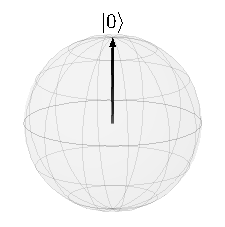
\includegraphics[width=0.8\linewidth]{chapter-1/zero}
    \end{minipage}%
    \begin{minipage}{0.23\textwidth}
        \centering
        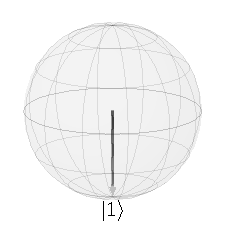
\includegraphics[width=0.8\linewidth]{chapter-1/one}
    \end{minipage}
    \begin{minipage}{0.23\textwidth}
        \centering
        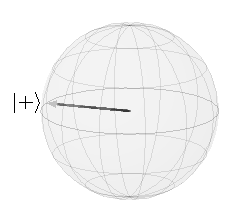
\includegraphics[width=0.89\linewidth]{chapter-1/plus}
    \end{minipage}
    \begin{minipage}{0.23\textwidth}
        \centering
        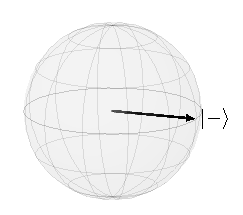
\includegraphics[width=0.89\linewidth]{chapter-1/minus}
    \end{minipage}
    \caption{Bloch sphere representations of orthonal computational basis states.}
\end{figure}

Whilst a single qubit can exist in an infinite number of states, upon measuring the qubit state with respect to a particular basis, the qubit state collapses into one computational basis state or the other. This gives rise to the \textit{no-cloning theorem}, which states that it is impossible to create an indentical and independent copy of an arbitrary unknown quantum state, as this would involve first measuring that state. This is one of the many ways in which quantum computation differs from classical computation.

Let us now consider systems consisting of multiple qubits. Similarly to how $n$ classical bits give rise to $2^n$ binary strings, $n$ qubits give rise to $2^n$ basis states. These basis states are formed by taking the Kronecker product of individual qubit states. For instance, a two-qubit system gives rise to four two-qubit basis states.
\begin{equation*}
    \ket{00} = \ket 0 \otimes \ket 0 \qquad
    \ket{01} = \ket 0 \otimes \ket 1 \qquad
    \ket{10} = \ket 1 \otimes \ket 0 \qquad
    \ket{11} = \ket 1 \otimes \ket 1
\end{equation*}
An arbitrary \textit{$n$-qubit state vector} describing the state of the entire system can be formed by taking a complex linear combination of the $2^n$ basis states. It follows that, in order to fully describe an arbitrary $n$-qubit state vector, we need to specify $2^n$ complex coefficients. In the case of a two-qubit system, we have the following.
\begin{gather*}
    \ket\psi =
    \alpha \ket{00} +
    \beta \ket{01} +
    \gamma \ket{10} +
    \delta \ket{11} \\
    \text{where} \,\,\,\, \alpha, \, \beta, \, \gamma, \, \delta \in \mathbb{C}
\end{gather*}

%%%

Quantum gates are, by definition, unitary transformations, $U^{-1} = U^\dagger$. In other words, a valid quantum gate corresponds to a square unitary matrix that conserves the complex inner product of the state that it acts on. In this way, quantum gates can be thought of as rotations of the qubit state vector in the Hilbert space.

We will now introduce the Pauli matrices, which are implemented on a quantum device as the Pauli gates. The Pauli gates are single-qubit gates that rotate their input by $\pi$ radians about in their respective basis. We define the Pauli matrices as the following $2 \times 2$ matrices.

\begin{figure}[H]
    \centering
    \begin{equation*}
        I = \begin{pmatrix} 1 & 0 \\ 0 & 1\end{pmatrix} \qquad
        X = \begin{pmatrix} 0 & 1 \\ 1 & 0\end{pmatrix} \qquad
        Y = \begin{pmatrix} 0 & -i \\ i & \,\,\,\,0\end{pmatrix} \qquad
        Z = \begin{pmatrix} 1 & \,\,\,0 \\ 0 & -1\end{pmatrix}
    \end{equation*}
    \caption{The four Pauli matrices.}
    \label{pauli-matrices}
\end{figure}


%%%

\subsection{Unitary Coupled Cluster Ansatz}%
\label{unitary-coupled-cluster-ansatz}

As suggested by Peruzzo \textit{et al} \cite{Peruzzo2014}, the UCC formulation of a wavefunction can be efficiently implemented on a quantum device in terms of quantum gates, whose implementation we refer to as the UCC ansatz $\ket{\psi(\bm\theta)}$. In other words, the UCC ansatz corresponds to some unitary excitation operator $U(\bm\theta)$ that acts on a reference state, usually a single reference Slater determinant Hartree-Fock state $\ket{\psi_0}$ obtained via the self-consistent field method.
\begin{equation*}
    \ket{\psi(\bm\theta)} = U(\bm\theta) \ket{\psi_0} =
    e^{\hat T(\bm\theta) - \hat T^\dagger(\bm\theta)} \ket{\psi_0}
\end{equation*}

The operator $\hat T(\bm\theta)$ is a linear combination of fermionic excitation operators, parametrised by coupled cluster amplitudes $\bm\theta$. The exponential of the anti-Hermitian operator $\hat T(\bm\theta) - \hat T^\dagger(\bm\theta)$ is therefore, by definition, unitary. 
\begin{equation*}
\hat T(\bm{\theta}) - \hat T^{\dagger}(\bm{\theta}) =
\sum_{i, a} \theta^a_i (a^\dagger_i a_a - a^\dagger_a a_i) + 
\sum_{i, j, a, b} \theta^{ab}_{ij} (a^\dagger_i a^\dagger_j a_a a_b - a^\dagger_a a^\dagger_b a_i a_j) + \dots
\end{equation*}

Where $i, j$ indexes occupied spin orbitals and $a, b$ indexes virtual, or unoccupied, spin orbitals. The resulting unitary operator $U(\bm\theta)$ cannot be directly implemented on a quantum computer since the terms of the excitation operator do not commute. Instead, we must invoke the Trotter formula to approximate the unitary. Taking a single Trotter step $\rho=1$, since our focus is on the NISQ setting \cite{Cowtan2020}, we define the UCC ansatz as the following product of $k$ parametrised unitary operators.

\begin{figure}[H]
    \centering
    \begin{equation*}
        \ket{\psi(\bm\theta)} = \prod_{m=1}^k U_m(\theta_m) \ket{\psi_0} \qquad
        U_m(\theta_m) = e^{\theta_m (\tau_m - \tau_m^\dagger)}
    \end{equation*}
    \caption{Parametrised $k$-UCC ansatz.}
\end{figure}

Where $m$ indexes all possible excitations and $\tau_m - \tau_m^\dagger$ corresponds to anti-Hermitian fermionic excitation operators in second quantisation. For the remainder of this thesis, we will refer to fermionic excitation operators $U_m(\theta_m)$ as the the exponentials of these anti-Hermitian operators. As these fermionic excitation operators derive from second-quantised operators, they preserve the fermionic anti-symmetry and particle number of the reference state.

The operators are then mapped to quantum gates (see Chapter \ref{excitation-operators}) before being implemented on a quantum device. It has been shown by Evangelista \textit{et al} \cite{Evangelista2019} that the UCC ansatz can exactly parametrise any state. Within the DISCO-VQE framework, we consider only generalised \textit{single} (one-body) and \textit{double } (two-body) fermionic excitation (operators), which as shown by Evangelista \textit{et al} \cite{Evangelista2019} achieves universality provided that we combine enough suitably-ordered one-body and two-body excitation operators \cite{Burton2023}. In other words, the UCCSD ansatz is sufficient to represent any vector in the Hilbert space.

\begin{figure}[H]
    \centering
    \begin{equation*}
    \hat T(\bm{\theta}) - \hat T^{\dagger}(\bm{\theta}) =
    \sum_{i, a} \theta^a_i (a^\dagger_i a_a - a^\dagger_a a_i) + 
    \sum_{i, j, a, b} \theta^{ab}_{ij} (a^\dagger_i a^\dagger_j a_a a_b - a^\dagger_a a^\dagger_b a_i a_j)
    \end{equation*}
    \caption{Truncated operator containing only \textit{single} and \textit{double} excitations.}
\end{figure}
